\section{Results}
\label{sec:results}

	% Methodology
	Para realizar uma avaliação ponderada dos custos de criar, executar
	e esperar uma tarefa, criamos um benchmark sintético que realiza a escrita
	nos endereços de uma página de memória, e.g., 4~KB. Para garantir 95\% de
	confiança, foram realizadas 50 replicações, descartando-se as primeiras 10
	para ignorar o período de aquecimento.

	Figura~\ref{tab:parameters}.
	\begin{table}[]
	\centering
	\caption{Benchmark parameters for experiments.}
	\label{tab:parameters}
	\begin{tabular}{llll}
	\toprule
			\textbf{Benchmark}   & \textbf{\#Tasks} & \textbf{\#Threads} & \textbf{Memory}                   \\
			\midrule
			Single Dispatcher    & 1 to 29          & 1                  & $1 \times 8~KB = 8~KB$            \\
			Multiple Dispatchers & 1 to 29          & 14                 & $14 \times 8~KB = 112~KB$         \\
			Threads              & 1 to 29          & 1 to 29            & $[1,29] \times 8~KB = [8,232]~KB$ \\
			\bottomrule
	\end{tabular}
	\end{table}


	A Tabela X exibe a aplicação deste benchmark replicado em três cenários
	diferentes:
	\begin{enumerate*}[label=(\roman*)]
		\item Um único dispatcher atende todas as tarefas sequencialmente;
		\item Cada núcleo escravo que esteja livre contém um dispatcher
			diferente atendendo tarefas paralelamente, resultando em 14
			dispatchers;
		\item Uma thread para cada tarefa, variando a quantidade de threads
			entre 1 à 29 threads.
	\end{enumerate*}
	A quantidade de Tarefas foi limitada a quantidade possível de threads
	simultâneas dentro do microkernel para que não fosse necessário replicar
	o comportamento de tarefas nas threads de usuário.
	% Experiments and Parameters
	É possível verificar também, além de exibir a quantidade the tarefas
	e threads envolvidas, a quantidade de memória necessária para execução de
	cada cenário.  Com base nisso, podemos perceber que muito qualquer esforço
	extra, o usuário pode utilizar a abstração de tarefas com dispatchers
	e manter a quantidade de memória utilizada limitada.
	%
	Especialmente, o cenário com um único dispatcher é a situação ideal para
	que o mesmo possa a proveitar o tempo ocioso do núcleo mestre mas este
	limita.

	A Figura B mostra os tempos de execução de cada cenário. Os tempos
	coletados são compostos do periodo de Dispatch/Create e Wait/Join de uma
	Tarefa/Thread.

	% Time
	Figura~\ref{fig:time}.
	\begin{figure}[]
			\centering
			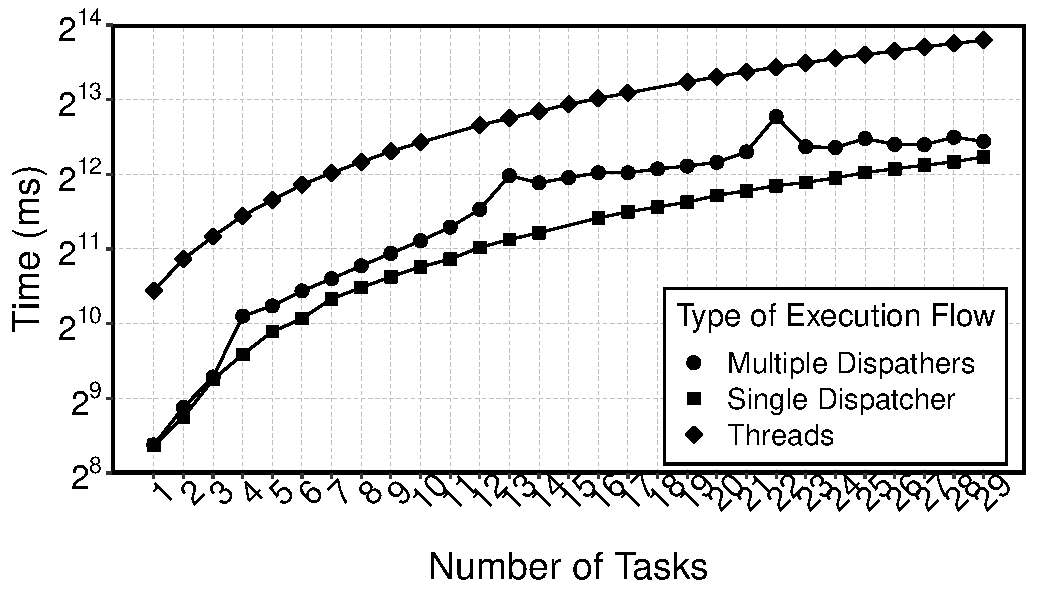
\includegraphics[width=0.90\linewidth]{tasks-time}
			\caption{Runtime Results.}
			\label{fig:time}
	\end{figure}
